% Chapter Template
\chapter{A Secure Bootstrapping for Constrained Devices} % Main chapter title

\label{Chapter5} % Change X to a consecutive number; for referencing this chapter elsewhere, use \ref{ChapterX}

\lhead{Chapter 5. \emph{A Secure Bootstrapping for Constrained Devices}} % Change X to a consecutive number; this is for the header on each page - perhaps a shortened title

%----------------------------------------------------------------------------------------
%	SECTION 5
%----------------------------------------------------------------------------------------

In previous chapters, we have presented a sort of security protocols allowing devices to discover, and to connect with each other within short physical range. These protocols are fundamentally important in systems where many various devices are co-working. A famous term denoting for the such systems is "Internet of Things" (IoT). Meanwhile, high amount of heterogeneous devices interoperating together in IoT link to many challenges on scalability, effectiveness, constrained resources, and security for both researching and industrial sectors. Additionally, many aspects of IoT have not standardised, especially security mechanisms. 

As one of the biggest challenges in IoT, secure bootstrapping for constrained things are exceptionally paid attention by researchers. The term bootstrapping denotes process of configuring a thing to properly participate in normal network operation~\cite{secureboot}. Bootstrapping is complete when a thing receives all settings such as an identity, secret keys, a list of access control, and protocol suits. Apparently, the setting information received in this stage is so sensitive that it indeed should be secured to maintain security and scalability of systems. However, existing traditional security solutions for both wired and wireless network are not feasible to tackle the problems. 

Based on mentioned enhanced security protocols and our formal method in previous chapters, we conduct a new complete secure bootstrapping scheme for resource-constrained things that focuses on security, robustness, adaptability, scalability, constrained resources. Precisely, we aim to these goals:
\begin{itemize}
\item Our scheme is sufficiently light to be deployed in constrained devices.
\item It works in case of unaccessible controllers.
\item Reused devices are welcome in our scheme.
\item Bootstrapping information is strictly considered on security.
\item Security analysis is offered. 
\end{itemize}

The rest of this chapter is organised as follows. The first section~\ref{5intro} introduces requirements for bootstrapping schemes for constrained things. Then, section~\ref{buildingblocks} discusses about secure bootstrapping building blocks and related work. In section~\ref{proposal}, we introduce our secure bootstrapping scheme for constrained devices in IoT. Section~\ref{validation} presents formal proofs. Finally, section~\ref{conclusion} concludes the chapter. 

\section{Bootstrapping Schemes and Requirements for IoT}\label{5intro}

Bootstrapping is a sequence introducing a new thing and enabling it to normally operate in a network. Apparently, securing bootstrapping process is essential at the first line of defence strategy. Traditionally, security bootstrapping approaches mainly adopt device pairing protocols, or key generation or distribution protocols. However, in the context of Internet of Things, since things are usually various types and resource-constrained devices, establishing a secure channel among devices remarkably costs time and efforts. The problem additionally enlarges when a controller and other things do not have any prior knowledge about a new thing.

In this chapter, we examine problems of secure bootstrapping in home network. The environment in which the bootstrapping scheme takes place includes these main factors:
\begin{itemize}
\item \textbf{A home gateway} playing as a center controller manages devices, checks origin of devices, synchronise to the cloud service.
\item \textbf{Cloud Sevice} playing as a remote controller allows users to remotely control their things. 
\item \textbf{Things} have some functions on providing services to users, and also autonomously configuring in the home network.
\item \textbf{A smartphone} playing as an introducer introduces a new device to the home network, and manages remotely the home gateway or the cloud.
\end{itemize}

The things are constrained devices such as light sensors, temperature sensors, smart TVs, smart fans, and so on. Some such these things definitely have limited computing power, limited amounts of memory, and simple interfaces such as a button, a LED light, or a light sensor. As disconnected to wired network, they communicate to others via wireless network. Furthermore, manufactories implant information into things in non-volatile memory. The information includes: a unique manufactory identification, a device identification, and a manufactory fingerprinting.

Smartphones and home gateway are assumed to have a trust relationship through secure TLS using pre-shared keys. Moreover, when the smartphone is accidentally lost, all its information stored the home gateway will be wiped out intermediately by users. Additionally, since attacker can exploit information stored in the smartphone, the smartphone is recommended to not contain any network group key, and things' information. 

As far as our concern, we study a secure bootstrapping scheme in circumstances (i) when a new thing has constrained interfaces and power, (ii) when the home gateway is replaced or out-of-order, and (iii) when a new thing is second-handed. Therefore, we state requirements for secure bootstrapping solutions for the Internet of Things as below.
\begin{enumerate}
\item [(i)] It must be secured against attacks on key agreements between a new thing and other things;
\item [(ii)] A solution should not only be intuitive for non-expert users but also be difficult for installers to introduce any vulnerability into target systems; 
\item [(iii)] The solution does not require a special additional setup hardware. The specialised hardware like ultrasound interfaces, or a large colour screen will significantly increase deployment cost. 
\item[(iv)] The heavy cryptographic algorithms should not be applied on constrained devices, e.g. public key algorithms. 
\end{enumerate} 

Since, no current proposal fulfils them, this motivates us to propose a new bootstrapping scheme which: 
\begin{itemize}
\item does not require implanted an one-time-password, or device certificates;
\item does not require a pre-shared key between devices and a home gateway;
\item does not require a public key infrastructure in home network;
\item enable to reuse or resale things; 
\item allows to bootstrap or rebootstrap in case of malfunction home gateways;
\item does not share network group keys between things and introducers;
\end{itemize}

We continues to deeply discuss these such building blocks and related work in the next section before we present our scheme. 

\section{Secure Bootstrapping Building Blocks}\label{buildingblocks}

Bootstrapping procedure normally can be split into three distinct building blocks~\cite{secureboot}: a pairing block, a registration block, and a network association block. Their functions are described as below. 
\begin{enumerate}
\item [(i)] The secure pairing block manages a thing to securely pair with an introducer; 
\item [(ii)] The registration block manages an introducer to provide registration information from a home gateway or registration services to a thing,
\item [(iii)] The network association manages a thing to join or to recommission to the network.
\end{enumerate}

In practice, a bootstrapping scheme can be constructed by either one, two, or full three these building blocks, e.g device pairing protocols are simple ones. Thus, we classify current approaches depending on these tasks, and address their limitations. 

\subsection{Pairing Block}
Recent studies concern on secure key sharing between a new thing and an introducer. The easiest way is using a QR code (abbreviated from Quick Response Code) consisting of a one-time-password either implanted at the manufactory site, e.g in~\cite{Jeanning2013}, or generated at the bootstrapping process, e.g in~\cite{Seung2015}. Then, the introducer uses a camera to extract information in QR codes. However, these methods meet a problem if QR codes are removed or lost, or if devices do not have a screen. Some alternatives adopt some kinds of out-of-band channels to securely transmit keys such as NFC, LED in\cite{4159919}, or human channels in~\cite{5654588}.

Another main approaches~\cite{JCMjcm0708634642, Cha:2011:LSE:1968613.1968679, Ikram:2009:SLA:1582379.1582583, 6263790} use pre-shared keys, or trusted public keys between a thing and a home gateway in 6LoWPAN~\cite{6lowpan} to establish secure channels. However, because of exchanged through secure channels, pre-shared keys are not sufficiently convenient for users when they have to deploy keys in a farm of things, and update keys for them. Alternative approaches use a PKI system to automatically deliver and to verify keys. The system apparently allows a home gateway to authenticate a new thing, but it is not truely friendly to constrained devices. 

Furthermore, it is clearly impossible for bootstrapping when the home gateway is disconnected to the network. Concerned as a solution, a trusted smartphone proposed in ~\cite{Seung2015},~\cite{6934398} can act as an authenticator. Nevertheless, losing phones is definitely painful to users since their phone are storing a bundle of sensitive information such as network keys, or authentication keys. 

\subsection{Registration Block}
Barely concerned in existing work, the device registration is partly built in device authentication schemes. However, in sensitive networks like home networks, new things must be authorised before joining. The device registration is, hence, required at the early step to avoid rogue or fake devices. 

Proposed in~\cite{Jeanning2013}, a mothership acting as a registration point verifies device status, and generates a device fingerprinting whenever an introducer or a home gateway requests. In the same approach, a service registration for Zigbee devices is proposed in ~\cite{5174409}.

Whereas standard protocols such as RADIUS~\cite{RADIUS}, PANA~\cite{rfc5191, Sarikaya2015}, EAP-TLS~\cite{eaptls}, HIP-DEX~\cite{hipdex} offer strong authentication and registration services, they are just useful if a new thing has obtained some common trusts , e.g. public keys, pre-shared keys, or trusted authentication servers.

\subsection{Network Association Block}
Generally, when successfully registered in a network, a thing has already obtained further configurations such as cluster head selection, routing protocols, or secure neighbour discovery protocols. Nonetheless, the way a new thing joins in the network is not presented clearly in current approaches. Otherwise, the thing might receive incorrect information, or association protocols contain undesired flaws. 

Furthermore, working in distributed environments, things can loose their connections occasionally. Instead of re-authentication, the things only need re-association using their authenticated materials such as session keys, or authenticated public keys. Some protocols such as GSAKMP~\cite{gsakmp}, GDOI~\cite{gdoi}, PANA~\cite{rfc5191}, EAP-TTLS~\cite{EAP-TTLSv0}, and MIKEY~\cite{MIKEY} offer association process, they are too heavy on constrained devices yet. 


\section{A Proposal For Secure Bootstrapping in IoT}\label{proposal}

Combining all above facts in the previous section, current approaches are aggressively debated to be adopted in context of Internet of Things. In this part, as far as concerning on our requirements and tackling the problems, we propose a novel secure bootstrapping scheme that offers lightness, robustness, adaptability, scalability and security. To begin with, we describe notations using in this chapter. 

\subsection{Notations}

In this chapter, the following notation presented in the table~\ref{notation} will be used. Note that, things in home sometime can be classified in groups based on their functionalities, so Dev\_Type is offered for this purpose. Moreover, ACL, abbreviated from access control list, denotes a set of permissions attached to a thing to identify services or operations allowed on given things. Dev\_Desc, or device description, describes in detail device information such as a device specification, a created date, a version, current firmware, and etc, and it is normally provided be manufactures. 

Provided and signed by a home gateway/a cloud service, a device fingerprinting, or Dev\_FR, available to each thing includes a device network address, a device DH key, a device type, and an expiration date. Whenever any piece of a device fingerprinting is required to change, the fingerprinting owner must contact to a controller via bootstrapping process. 

Provided by a home gateway/a cloud service, Net\_CONF is network settings containing network identification, an access control list, and a network address of a home gateway. Thus, these information enable a thing to maintain normal operations in the network. Due to undesired replacement of inner information, Net\_CONF is apparently signed by the home gateway private key. 

A network group key, or NetPass, plays an important role to offer a cryptographic material for establishing secure communications among authorised things. Thus, introducers should not store these information if it is not one of authorised things in the home network. Otherwise, compromised or lost introducers are potential threats to the system. Additionally, each NetPass includes a sequence number, or ID, allowing things to update keys when their NetPass is obsoleted. Shared keys, or KS, established during pairing or association process are a combination of two device DH keys. 

\begin{table}[t]
\centering
\caption{\textsc{Notations}}
\label{notation}
{\small
\begin{tabular}{| l | p{9cm} |}
 \hline
\emph{MS\_ID} & 32-bit unique manufactory identification. \\ \hline
\emph{Dev\_ID} & 32-bit device identification. \\ \hline
\emph{MS\_FR} & manufactory fingerprinting used by third-party services to verify manufactories. \\ \hline
\emph{Dev\_Type} & device type chosen by the user \\ \hline
\emph{Dev\_Status} & the status of a device including sold, registered, unregistered, or brand-new \\ \hline
\emph{Dev\_Desc} & information describing device specification. \\ \hline
\emph{Dev\_Key} & the device DH key generated in secure pairing process \\ \hline
\emph{Dev\_URN} & the unique URN assigned by the manufactory to uniquely identify the device. \\ \hline
\emph{Dev\_Addr} & the network address of the device \\ \hline
\emph{Expires} & the expiration date of device fingerprinting \\ \hline
\emph{SH\_PrKey} & the home gateway's private key \\ \hline
\emph{Dev\_FR} & device fingerprinting formed as \\
 & $\{Dev\_Addr, Dev\_Key, Dev\_Type, Expires\}_{SH\_PrKey}$ \\ \hline
\emph{Dev\_Info} & the device information including $MS\_ID$, $Dev\_ID$, $MS\_FR$, and $Dev\_URN$ \\ \hline 
\emph{SH\_Addr} & the network address of the home gateway \\ \hline
\emph{Net\_ID} & the home network ID \\ \hline
\emph{ACL} & the access control list \\ \hline
\emph{Net\_CONF} & the network settings including $Net\_ID$, $ACL$, $SH\_Addr$ provided by the home gateway \\ \hline
\emph{NetPass} & the network group key including $\{Key,ID\}_{SH\_PrKey}$ where $ID$ is a sequence number of the $Key$ \\ \hline
\emph{KS} & the shared key between things, or things and smartphones \\ \hline
\emph{SH\_PbKey} & the home gateway's public key \\ \hline
$--$ & dashed line describing an out-of-band channel or a secure channel \\ \hline
 \end{tabular}
}
\end{table}
 
\subsection{Overview}

Our general bootstrapping scheme is illustrated at the figure~\ref{bootscheme}. The scheme contains a set of protocols enabling a new thing to completely participate in an existing authenticated home network. A new thing receives a set of information at manufactory via a secure channel. We assume that attackers cannot violate this process. To begin a bootstrapping process, a thing needs an introduction from a trusted smartphone. After establishing a secure channel via secure pairing process, the smartphone receives all thing's information including a thing's DH key. The smartphone then opens a secure TLS channel to a home gateway/a cloud service to this information. The home gateway/ cloud service validates the thing using its manufactory identification, and device URN (Uniform Resource Name). After successful registration, the home gateway/ cloud service receives device information and current device status. The home gateway/the cloud service produces a device fingerprinting and network configuration and offers them to the thing via the smartphone. Finally, the new thing launches network association process with an authorised thing to participate in the home network. 

\begin{figure*}
  \centering
  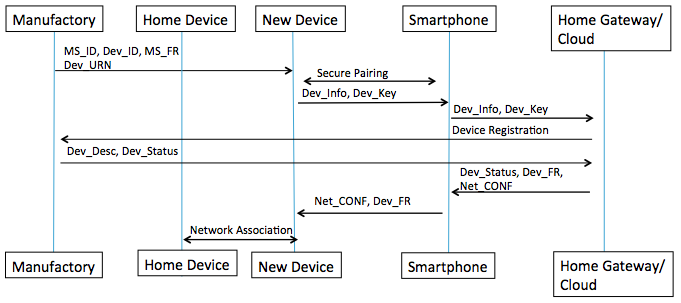
\includegraphics[width=1\textwidth]{boot}
  \caption{Secure Bootstrapping Scheme}
  \label{bootscheme}
\end{figure*}

\subsection{Attack Model}
Attackers' goals are cracking down key agreements between things and home gateways, registration servers, or smartphones. Since our proposed solution adopts multiple communication channels, the penetrator model is refined to capture both Dolev-Yao attacks on open channels such as wireless, or power line, and attacks on secure channels defined in chapter 3. In particular, Dolev-Yao penetrators can overhear, intercept, modify and inject arbitrary messages into public medium while limited capabilities, e.g. overhearing, dropping, delaying, replaying, and forwarding messages on sorts of secure channels. 

\subsection{Pairing Process}

Pairing process aims to create a secure communication between a new thing and a smartphone. It is mainly based on our proposed protocol in~\ref{chap42move}. And according to our proof, this protocol could achieve strong security even with a low-bandwidth OOB channel. 

\begin{figure}
  \centering
  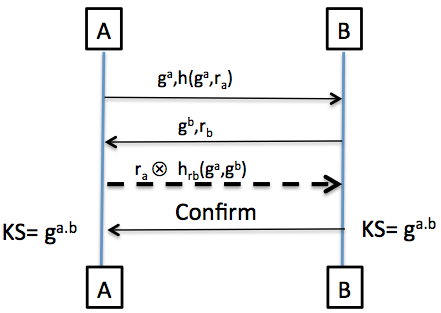
\includegraphics[width=0.5\textwidth]{pairing}
  \caption{Secure Device Pairing Protocol}
  \label{devicepairing}
\end{figure}

The protocol is depicted in the figure ~\ref{devicepairing} and presented as follows. 
\begin{enumerate}
\item The new thing and the smartphone generate its own device key $g^a$ and $g^b$ correspondingly. 
\item The new thing picks a random value $ra$. The smartphone picks a random value $rb$
\item The new thing sends $(g^a,h(g^a,ra))$ to the smartphone. The smartphone records $g^a$ as Dev\_Key of the new thing. 
\item The smartphone sends $(g^b,rb)$ to the new thing.
\item The new thing sends $(ra \oplus h_{rb}(g^a,g^b) )$ to the smartphone over a public out-of-band channel. 
\item The smartphone verifies received values and announces the result to the new thing. 
\item The new thing confirms by pushing an Accept button. 
\item Both side generate the shared key $KS = g^{a.b}$
\item The new thing sends encrypted information including manufactory identification, device identification, manufactory fingerprinting, and device URN using KS to the smartphone. 
\end{enumerate}

\subsection{Registration Process}

The registration process happens between a smartphone and a home gateway/a cloud service. In this step, the new thing wishes to be validated and to securely receives a device fingerprinting and network settings. The process starts after the smartphone receives a bunch of information from the new thing including $MS\_ID$, $Dev\_ID$, $MS\_FR$, and $Dev\_URN$ in previous step. The smartphone enrols the new thing to the home gateway. The protocol is illustrated at the figure~\ref{registration}, and presented as below.
\begin{enumerate}
\item The smartphone opens a secure TLS connection to the home gateway using a pre-shared key.
\item The smartphone sends all device information, a device type, and the device's DH key to the home gateway. 
\item The home gateway validates the device information to the manufacture  over a secure HTTPS connection. 
\item The manufactory sends the $Dev\_Desc$ and $Dev\_Status$ to the home gateway.
\item The home gateway possible requests a device registration to the manufactory site if the device has not been registered. 
\item After successful validation and registration, the home gateway generates the $Dev\_FR$, then sends $Dev\_FR$, $Net\_CONF$, $Dev\_Status$, and $SH\_PbKey$ to the smartphone. Furthermore, depending on $Dev\_Type$, an access control list $ACL$ in $Net\_CONF$ is selectively generated by the home gateway.
\item The smartphone offers $Net\_CONF$, $Dev\_FR$, and $SH\_Pub$ to the new thing.
\item The smartphone cleans all received information when completing the process. 
\end{enumerate}

In case of inaccessible home gateway, the smartphone can forward the registration process to the cloud service as a remote controller. The cloud service then updates new information to the home gateway whenever it is available. 
\begin{figure}
  \centering
  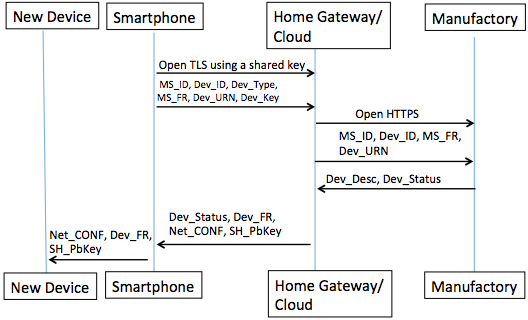
\includegraphics[width=0.94\textwidth]{verification}
  \caption{Registration Process}
  \label{registration}
\end{figure}

\subsection{Association Process}

Network association happens between an authenticated thing(A) and an authorised thing(B). The purpose of this process is exchanging the network group key or creating a per-neighbour key between two devices. In this thesis, we design a network group key exchange.

$A$ wishes to receive the network group key, or NetPass, from $B$. The protocol is illustrated in the figure~\ref{netasso}, and happens as follows. In this figure, we denote $Dev_{A}\_FR$ as A's fingerprinting, and $Dev_{B}\_FR$ as B's one. $Dev_{A}\_ID$ and $Dev_{B}\_ID$ denote A's identification and B's identification correspondingly. $g^a$ and $g^b$ are DH keys generated at the pairing process. Apparently, each value is linked to a corresponding device fingerprinting. 

\begin{enumerate}
\item After neighbour discovery process by sending Hello messages, $A$ offers $g^a, Dev_{A}\_FR$ to $B$. 
\item $B$ provides its device fingerprinting $g^b,Dev_{B}\_FR$ to $A$. Then both sides validate their fingerprinting using the public key of the home gateway. 
\item Both sides produce a shared key $KS = g^{a.b}$. 
\item $A$ generates a nonce $r_a$, then sends $\{r_a, Dev_{A}\_ID\}_{KS}$ to $B$.
\item $B$ sends $\{r_a,r_b,Dev_{B}\_ID, NetPass\}_{KS}$ to $A$. 
\item $A$ sends back $\{r_b\}_{KS}$.
\end{enumerate}

\begin{figure}
  \centering
  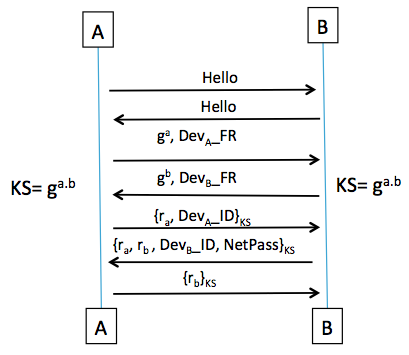
\includegraphics[width=0.5\textwidth]{networkasso}
  \caption{Network Association}
  \label{netasso}
\end{figure}

Note that, it is possible for a home gateway playing in role of an authorised thing. 

\subsection{Reassociation and Network Key Updating}
 
Unlike the association process, the reassociation happens between two authorised things $A$ and $B$. In particular, they wishes to exchange their $NetPass$ securely. When one thing receives a $NetPass$ from the other, it checks the $NetPass$'s $ID$. If the new $ID$ is bigger than its current $NetPass$ ID, then the thing will update its $NetPass$ key. The protocol is presented below and illustrated at the figure~\ref{renetasso}.

\begin{enumerate}
\item After neighbour discovery process by sending Hello messages, $A$ offer $g^a, Dev_{A}\_FR$ to $B$. 
\item $B$ provides its device fingerprinting $g^b,Dev_{B}\_FR$ to $A$. Then both sides validate their fingerprinting using the public key of the home gateway. 
\item Both sides produce a shared key $KS = g^{a.b}$. 
\item $A$ generates a nonce $r_a$, then sends $\{r_a, Dev_{A}\_ID\}_{KS}$ to $B$.
\item $B$ sends $\{r_a,r_b,Dev_{B}\_ID, NetPass1\}_{KS}$ to $A$. 
\item $A$ sends back $\{r_b,NetPass2\}_{KS}$.
\end{enumerate}

\begin{figure}
  \centering
  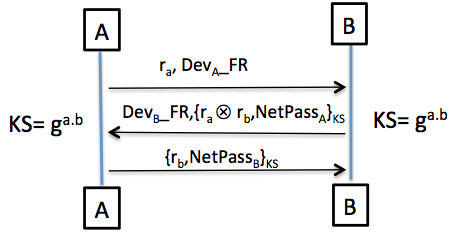
\includegraphics[width=0.5\textwidth]{renetasso}
  \caption{Network Reassociation}
  \label{renetasso}
\end{figure}

By the way of reassociation, whenever a home gateway wishes to update the $NetPass$, it just disconnects and reassociates to neighbour things. Straightforwardly, the new $NetPass$ will be spread out to whole network via the reassociation process in each thing. 

\subsection{Reboostrapping}

Rebootstrapping supports re-authentication and rekeying for things, and allows things to be administratively switched to a different domain. Therefore, rebootstrapping always requires a smartphone. Whenever rebootstrapping process is demanded by a thing, the secure pairing process will be established between the thing and the smartphone. After pairing properly, the smartphone chooses a device type then runs the registration process. The home gateway regenerates the device's fingerprinting, then sends $Dev\_Status$, $Dev\_FR$, $Net\_CONF$, and $SH\_PbKey$ to the thing via the smartphone. 
 
\section{Security Analysis}\label{validation}

In this section, we present a sketch of proofs of our bootstrapping scheme since this scheme consists of some already-proved protocols.

Our proposed bootstrapping scheme aims to (i) key agreement between a new thing and a smartphone in device pairing process (ii) agreement on device fingerprinting between a new thing and a home gateway in the registration process (iii) network group key agreement between an authenticated thing and an authorised one in association process. 

\begin{Proposition}\label{ntandsp}
The new thing and the smartphone agree on the shared key $K= g^{a.b}$ if the smartphone is not compromised. 
\end{Proposition}

\begin{proof}

According to the assumption on the uncompromised smartphone, this secure pairing protocol is clearly proved in our last work~\ref{proof2step}. We also showed that the successful attack probabilities is $Pr[attack] \leq n.\gamma.2^{-k}$ where $n$ is the number of participants on the network, $\gamma$ is the maximum number of sessions for each participant, $k$ is the length of short authenticated string.
\end{proof}

\begin{Proposition}\label{newandsh}
A new thing and a home gateway agree on a device fingerprinting $Dev\_FR = \{Dev\_Addr, Dev\_Key, Dev\_Type, Expires\}_{SH\_PrKey}$. 
\end{Proposition}

\begin{proof}

According to the assumption on uncompromised shared key between the smartphone and the home gateway, attackers cannot open a secure connection to the home gateway/the cloud service with a fake key. Therefore, all messages transmitted on this connection are secured. As a result of this, only regular smartphone can get the device fingerprinting generated by the home gateway/the cloud service. 

Using the result of the proposition~\ref{ntandsp}, whenever a new thing gets a device fingerprinting from a regular smartphone, it can ensure this value produced by the home gateway/the cloud service. However, when the thing might contacts to attackers, the home gateway does not authenticate this thing. Moreover, while a legitimate fingerprinting is always signed by the home gateway's private key, the fake one cannot be validated at association process. 

\end{proof}

\begin{Proposition}
An authenticated thing(A) and an authorised thing(B) agree on $NetPass$. 
\end{Proposition}

\begin{proof}

Intuitively, both sides agree on the shared key $KS = g^{a.b}$ by following facts. 
\begin{enumerate}
\item [(i)] The proposition~\ref{newandsh} says the agreement on $Dev_{A}\_FR$ between A and a home gateway.
\item [(ii)] In case of faked smartphones, $A$ might obtain a fake device fingerprinting generated by attackers. However, by the assumption on uncompromised home gateway's private keys, $B$ is able verify $Dev_{A}\_FR$ if it is generated by the home gateway or not. 
\item [(iii)] According to the assumption on uncompromised $B$, $A$ is able to verify $Dev_{B}\_FR$. 
\end{enumerate}

Thus, after third and fourth messages, two principals own the same shared key $KS = g^{a.b}$. Additionally, since three last messages are a variant of $Needham$ $Schroeder$ protocol proved in~\cite{674832} using a pre-shared key, $A$ and $B$ can ensure the agreement on $Na$ and $Nb$. 
Moreover, encrypted by $KS$ in the sixth message, $NetPass$ cannot be obtained by any attacker. Therefore, $A$ is able to ensure secrecy of $NetPass$. Finally, both sides agree on the secured $NetPass$. 
\end{proof}

\section{Conclusion}\label{conclusion}

Obviously, not only does our scheme satisfy all of our mentioned requirements, it also provides unique features helpful to bootstrapping things in some sensitive circumstances. Compared to our scheme, current proposed schemes do not provide the same fashion in term of robustness, adaptability and scalability. Particularly, pairing methods such as ~\cite{4159919} and ~\cite{5654588} do not support authorisation and rebootstrapping. In~\cite{Seung2015, Jeanning2013}, QR codes containing an initial key could introduce a weakness point for the system if they are lost. Alternative solutions using pre-shared keys in \cite{JCMjcm0708634642, Cha:2011:LSE:1968613.1968679, Ikram:2009:SLA:1582379.1582583, 6263790, rfc5191} are not sufficiently convenient to users. Finally, lost smartphone in schemes ~\cite{Seung2015, 6934398} leads to leak sensitive information such as pre-shared keys, rebootstrapping information.

Eventually, this chapter offered a novel secure bootstrapping scheme for constrained devices in context of Internet of Things. Precisely, it takes advantage of unsupporting a PKI system, pre-shared keys, and pre-implanted keys. Furthermore, our scheme is not error prone to users since users only participate in the pairing process. Additionally, we attached the formal proofs. In close future, we continue implementing remaining parts of our bootstrapping scheme, and evaluate its usability.






